\subsection{Logical View}
Logical View skal danne et overblik over hvilke softwarepakker der befinder sig på platforme. Blokkene inde i de respektive pakker kan sammen med domænemodellen, hjælpe med at give et overblik over hvilke klasser og kernemoduler der skal bruges.
% Logical View Devkit8000
\subsubsection{Logical View Devkit8000}
\begin{figure}[H] \centering
    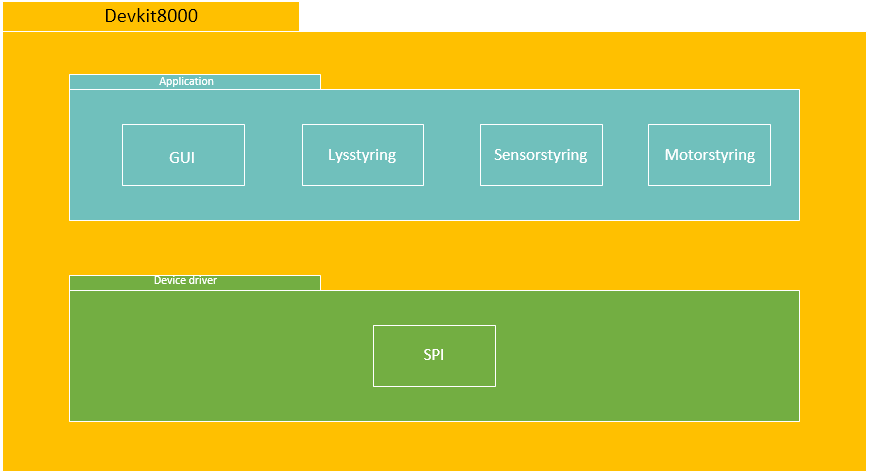
\includegraphics[width=\textwidth]{0_Filer/Figuer/LogicalViewDevkit8000.png}
    \caption{Logical View Devkit8000}
    \label{fig:LogicalView}
\end{figure}
Figur \ref{fig:LogicalView} illustrerer hvilke softwarepakker der ligger på Devkit8000. I bunden er Hardware API-pakken som håndterer protokol-vedtægter ifm. kommunikationen. I midten ligger Device drivers-pakken som håndterer protokol kommunikationen mellem Devkit8000 og PSoC. Application-pakken tager sig af alt UI samt kalibrering, sensorstyring og motorstyring.

% Logical View PSoC
\subsubsection{Logical View PSoC}
\begin{figure}[H] \centering
    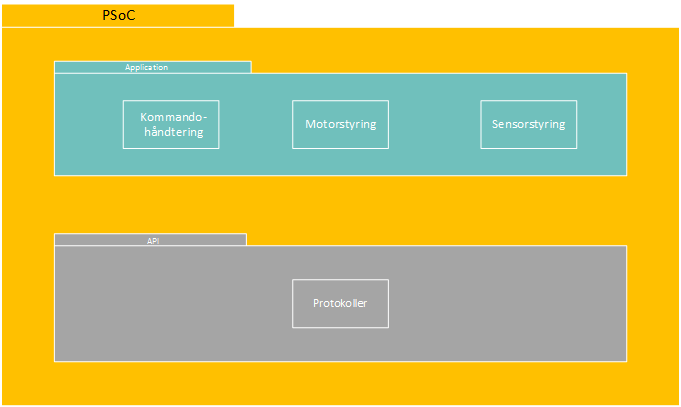
\includegraphics[width=\textwidth]{0_Filer/Figuer/LogicalViewPSoC.png}
    \caption{Logical View PSoC}
    \label{fig:LogicalViewPSoC}
\end{figure}
Figur \ref{fig:LogicalViewPSoC} illustrerer hvilke softwarepakker der ligger på PSoC. I bunden er en API-pakke som håndterer protokol-vedtægter ifm. kommunikationen. Øverst er application-pakken der tager sig af alt kommandohåndtering, motorstyring og sensorstyring.